A seguito di una prima parte teorica introduttiva, si procede in questo capitolo con la presentazione 
dell'impostazione pratica che si è voluto dare alle sperimentazioni condotte. La struttura secondo la quale verranno esposte 
le informazioni nei seguenti paragrafi ricalca la partizione logica alla base del codice sviluppato, pragmaticamente diviso 
in quattro moduli tra loro indipendenti:
\begin{itemize}
    \item Generazione dei parametri
    \item Generazione delle istanze di problemi MIP
    \item Risoluzione delle istanze di problemi
    \item Estrazione ed analisi dei risultati
\end{itemize}




\section{Generazione dei parametri}
Il primo problema presentatosi è stato quello relativo all'individuamento dei parametri di flusso e distanza, in quanto 
fondamentali per la creazione di istanze del problema e conseguentemente anche per la loro risoluzione.

La prima possibilità valutata è stata la generazione di valori casuali per comporre le matrici dei parametri $A$ e $B$. 
Questa però è stato scartata fin da subito poichè utilizzare valori di tale tipologia non permette di fornire una versione 
pseudo-realistica di istanze del problema ed inoltre, non garantisce alcun tipo di uniformità nella generazione delle istanze, 
il che non ci permette di effettuare successivamente uno studio approfondito sulla loro complessità di risoluzione.

La soluzione a questo problema è stata individuata in un metodo illustrato in un articolo del professor Éric D. Taillard del 1995
\cite{TAILLARD}. Come verrà illustrato più nello specifico nella prossima sezione, il metodo utilizzato è detto Densità di
grigio, in inglese (\textit{Density of grey}). Esso, oltre a compensare i difetti del metodo di istanziamento casuale, permette
di automatizzare la creazione delle matrici dei parametri realizzando un algoritmo che richiede ai fini della generazione 
esclusivamente due valori: dimensione dell'istanza e densità utilizzata.

Come anticipato nell'introduzione, per realizzare tale processo è stato fatto uso del linguaggio di programmazione \textit{Python} 
\cite{python} e come supporto \textit{NumPy} \cite{NumPy}, una libreria open source che aggiunge supporto a grandi matrici 
e array multidimensionali insieme a una vasta collezione di funzioni matematiche di alto livello per poter operare efficientemente 
su queste strutture dati.

\subsection{Istanze Tai*c}
Le istanze Tai*C, la cui denominazione deriva dal nome del loro ideatore, sono una particolare classe di problemi di assegnamento quadratico
che si fondano sull'utilizzo del metodo di Densità di grigio, il quale può essere descritto nel seguente modo.

Al fine di ottenere una tonalità di grigio di densità pari a $m/n$ , il metodo in questione consiste nel generare una griglia 
rettangolare contenente $n = n_1 \times n_2$ caselle quadrate, $m$ delle quali sono nere e $n-m$ sono bianche. 
Giustapponendo molte di queste griglie è possibile ottenere una superficie grigia di gradazione pari a $m/n$.
Per ottenere la miglior qualità di colore, è necessario che le caselle nere, o quelle bianche, siano sparse uniformemente nella griglia.

A prova di ciò viene qui riportata un'applicazione del metodo realizzata con una delle soluzioni ottenute.
\begin{figure}[h!]
    \centering
    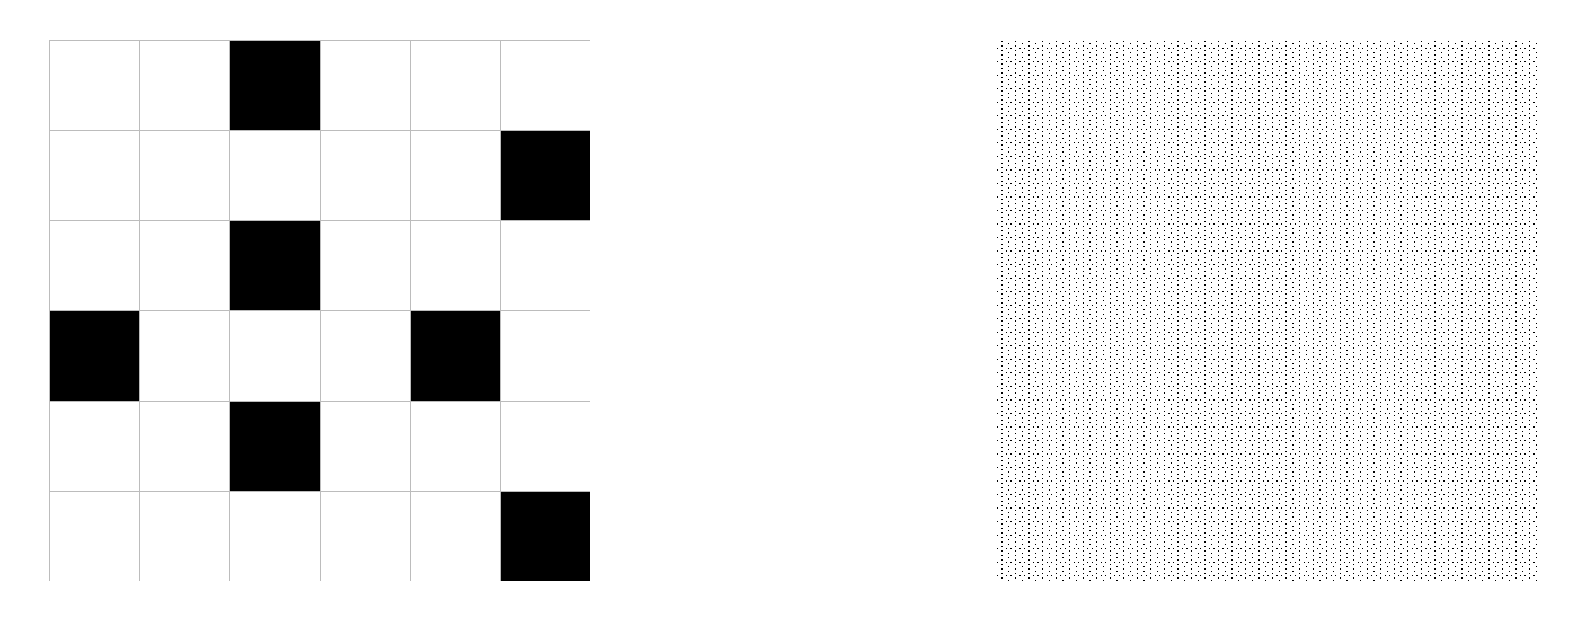
\includegraphics[scale=0.21]{images/Density_of_Grey.png}
    \caption{a sinistra la griglia relativa ad una soluzione ottima di un'istanza \textit{Tai36c} a densità $d=30\%$, 
             \newline a destra quella ottenuta accostando $1600$ griglie del tipo a sinistra}
    \label{fig:dnsgry}
\end{figure}

Per rendere al meglio l'idea che sta alla base del metodo, è possibile paragonare le caselle nere a degli elettroni e la griglia 
allo spazio accessibile agli elettroni. Il posizionamente di quest'ultimi deve essere effettuato in modo tale che la somma delle 
intensità delle forze di repulsione elettrostatica è minimizzata.

Nei problemi considerati, le forze $f_{rstu}$ $\(r,t \in \[1,n_1\] \; s,u \in \[1,n_2\]\)$ presenti tra le caselle $i$ e $j$
locate rispettivamente nelle posizioni della griglia di coordinate $\(r,s\)$ e $\(t,u\)$ sono definite come segue:
\begin{align*}
    f_{rstu} \, = \, \max_{v,w \,\in\, \{-1,0,1\}} \frac{1}{\(r-t+n_1 v\)^2 + \(s-u+n_2 w\)^2}
\end{align*}

Per ottenere una densità di grigio pari a $m/n$ è possibile risolvere un problema di tipo $QAP$ (assegnamento quadratico) in cui 
i parametri sono definiti nel seguente modo.
\begin{align*}
    a_{ij} \, = \, \begin{cases} 1 & \mbox{if } i \leq m \mbox{ and } j \leq m \\ 0 & \mbox{otherwise} \end{cases} 
    \qquad \;\;
    b_{ij} \,=\, b_{\; n_2 \(r-1\)+s \;\; n_2\(t-1\)+u} \,=\, f_{rstu}
\end{align*}

La $i$-esima componente $\(i\leq m\)$ di una soluzione $\pi$, $\pi_i = \pi_{n_2 \(r-1\)+s}$ fornisce la posizione in cui
deve essere posizonata una casella nera.

Nonostante la relativa semplicità di questi problemi, molti metodi risolutivi potrebbero non funzionare correttamente a causa 
dell'esistenza di più soluzioni con lo stesso valore obiettivo. Tali soluzioni posso essere ottenute scambiando la posizione 
di due caselle nere oppure attuando rotazioni, traslazioni o simmetrie delle caselle nella griglia. Queste tre infatti,
sono azioni che non mutano il valore della soluzione associata.

Questi problemi sono identificati in letteratura dalla sigla $grey$n$_1\_$n$_2\_$m e sono stati risolti pseudo-ottimamente 
fino a valori $n_1 = n_2 = 8$. Scegliendo definizioni dei parametri di distanza differenti oppure variando le scelte prese sui 
valori $n_1$, $n_2$ ed $m$ è possibile ottenere moltissime varianti del problema.

A questo punto è possibile sfruttare le definizioni degli elementi che caratterizzano questo modello, per realizzare degli algoritmi 
che generino la matrice dei flussi $A$ e quella delle distanze $B$ sulla base dei soli tre parametri richiesti, le dimensioni $n_1$ e $n_2$ 
(si ricorda queste sono in relazione con la dimensione dell'istanza $n$ nel seguente modo: $n=n_1\times n_2$) e la densità di grigio 
utilizzata $d$. 

Qui di seguito sono riportati gli pseudocodici degli algoritmi in questione insieme a quello delle eventuali funzioni che sono state 
utilizzate all'intero di essi.

\begin{algorithm}
    \caption{Matrix A generation}\label{A_gen}
    \begin{algorithmic}[1]
    \Function{A-generator}{$n, \,d$}
    \State $* \quad sia\; A = \[a_{ij}\] \quad *$
    \State $m \gets round\(n\cdot \(d/100\)\)$
    \ForAll{$i \in [0,n)$}
    \ForAll{$j \in [0,n)$}
        \If{$i<m \;\text{or}\; j<m$} \State $a_{ij} \gets 1$
        \Else \State $a_{ij} \gets 0$
        \EndIf
    \EndFor
    \EndFor
    \Return $A$
    \EndFunction
    \end{algorithmic}
\end{algorithm}

\begin{algorithm}
    \caption{Matrix B generation}\label{B_gen}
    \begin{algorithmic}[1]
    \Function{Force}{$n_1,\, n_2,\, r,\, s,\, t,\, u$}
    \State $max \gets 0$
    \ForAll{$v \in \{-1, 0, 1\}$}
    \ForAll{$w \in \{-1, 0, 1\}$}
        \State $m \gets 1\,/\(\(r-t+n_1 v\)^2 + \(s-u+n_2 w\)^2\)$
        \State $max \gets \max \(max, m\)$
    \EndFor
    \EndFor
    \Return $max$
    \EndFunction
    \BState
    \Function{B-generator}{$n_1,\, n_2$}
    \State $* \quad sia\; B = \[b_{ij}\] \,con \;valori \;inizializzati \;a \;zero \quad *$
    \State $scale \gets 100000$
    \ForAll{$r \in [0,n_1)$}
    \ForAll{$s \in [0,n_2)$}
    \ForAll{$t \in [0,n_1)$}
    \ForAll{$u \in [0,n_2)$}
        \State $i \gets n_2 \cdot \(r-1\)+s$
        \State $j \gets n_2 \cdot \(t-1\)+u$
        \If{$b_{ij} \, \neq \, 0$} \State continue
        \Else 
            \State $b_{ij} \gets \text{round} \(\text{Force}\(n_1,n_2,r,s,t,u\)\cdot scale\)$
            \State $b_{ji} \gets b_{ij}$
        \EndIf
    \EndFor
    \EndFor
    \EndFor
    \EndFor
    \Return $B$
    \EndFunction
    \end{algorithmic}
\end{algorithm}

Come si può intuire osservando lo pseudocodice del primo algoritmo, nella sua costruzione è stata presa la decisione di 
esprimere la densità $d$ in punti percentuali, ovvero $d \in \[0,100\]$. Da qui il perchè nel calcolo del valore di $m$ è necessaria 
la divisione per $100$.

Relativamente al secondo algoritmo invece, sono necessarie alcune puntualizzazioni. Alla riga n°10 si può notare come il valore della distanza 
calcolata tramite la funzione \textit{Force} non avviene direttamente ma vengono effettuate delle operazioni intermedie. Come prima cosa 
il valore ritornato dalla funzione viene scalato di un fattore \textit{scale} pari a $100000$ e successivamente viene arrotondato all'intero 
più vicino. In tale modo è stato possibile confrontare le matrici ottenute, nello specifico la \textit{Tai64c} e la \textit{Tai256c}, 
con quelle messe a disposizione dal sito web \textit{QAPLIB} \cite{QAPLIB}, una libreria online contenente diverse tipologie di istanze 
di prolemi di assegnamento quadratico tra cui la \textit{Tai*c}. Quest'operazione ha permesso in fase di costruzione dell'algoritmo di 
garantirne la correttezza. All riga n°21 invece, si sfrutta la proprietà di simmetria della matrice $B$ per risparmiare 
metà dei calcoli dei valori di distanza, riducendo così la complessità temporale dell'algoritmo. Si ricorda infatti che, date due unità 
qualsiasi, la distanza della prima dalla seconda è la medesima della seconda dalla prima.

Come si può notare sono state utilizzate due funzioni di cui non è stato riportato lo pseudocodice, \textit{max} e \textit{round}.
Questo perchè sono due funzioni elementari messe a disposizione della libreria standard di \textit{Python} \cite{python} di cui il 
funzionamento è noto. La prima richiede due valori come parametri e ritorna il massimo tra questi mentre la seconda ritorna 
l'arrotondamento all'intero più vicino del numero fornito come parametro.

\section{Generazione delle istanze di problemi MIP}
prova

\subsection{Modellazione algebrica}
prova

\subsection{Linearizzazione del modello}
prova

\subsection{Semplificazione del modello}
prova

\subsection{Modellazione nel software}
prova




\section{Risoluzione delle istanze di problemi}
prova




\section{Estrazione ed analisi dei risultati}
prova